\subsection{Comparing AdaptUI with other \ac{aui} Solutions}
\label{sec:imhotep_comparison}

As a second part of the technical evaluation, in this section a comparison 
between AdaptUI and Imhotep is performed. The purpose of this section is to 
demonstrate that the capabilities of the AdaptUI platform improve the ones 
provided by the Imhotep framework. Hence, this section is organized as follows: 
First, in Section~\ref{sec:imhotep_vs_adaptui} the Imhotep framework and its 
main characteristics is introduced. Next, a use case using both adaptation 
platforms is detailed (see Section~\ref{sec:assisted_city_use_case}). Finally, 
in Section~\ref{sec:imhotep_discussion} and Section~\ref{sec:imhotep_conclusions} 
a discussion and several conclusions are presented.

\subsubsection{Imhotep}
\label{sec:imhotep_vs_adaptui}

As mentioned in Section~\ref{sec:background_imhotep}, 
Imhotep~\citep{almeida_imhotep_2011} is a framework developed and maintained at
the University of Deusto which aims to ease the development of adaptable and 
more accessible user interfaces. The framework allows to develop applications 
without considering a specific design for the user interface, as it is built
from the definition of a series of preprocessor directives which evaluate a
user's and device's profile.

In order to fully understand how Imhotep works, Figure~\ref{fig:imhotep_architecture}
illustrates its architecture design. As can be seen in the figure, Imhotep is
divided into 4 modules:

\begin{itemize}
    \item The first one is the Application Downloader, which is a tool installed
    in the user's device to connect to the repository and download adapted
    applications.
    
    \item The \ac{rest} server contains the application repository. Once a user 
    selects a desired application, the server will:
    
    \begin{itemize}
      \item Use the Fuzzy Knowledge-Eliciting Reasoner to infer new values with
      the user and device configuration and the variables and rules established
      by the developer of the application.
      
      \item Call the Preprocessor to select only the code that the final user
      requires.
      
      \item Delegate the compilation of the application to the Compiler Manager.
      Currently the \ac{rest} server only supports Android, but other compilers could
      be easily added.
      
      \item Store the compiled application in the Compilation Cache, so future
      requests will not require to pass through the whole process if they have
      the same configuration values.
    \end{itemize}
    
  \item The Wizard: developers use the wizard to establish the variables and the
  possible values of those variables. It uses the trends database to show the
  different values given a concrete user and a concrete device.
  
  \item The Capacity Tester. Users have to create a user profile with their
  capabilities. The Capacity Tester will gather those capabilities by testing
  them. The Current application is just a proof of concept of how the Capacity
  Tester should work.
\end{itemize}

\begin{figure}
\centering
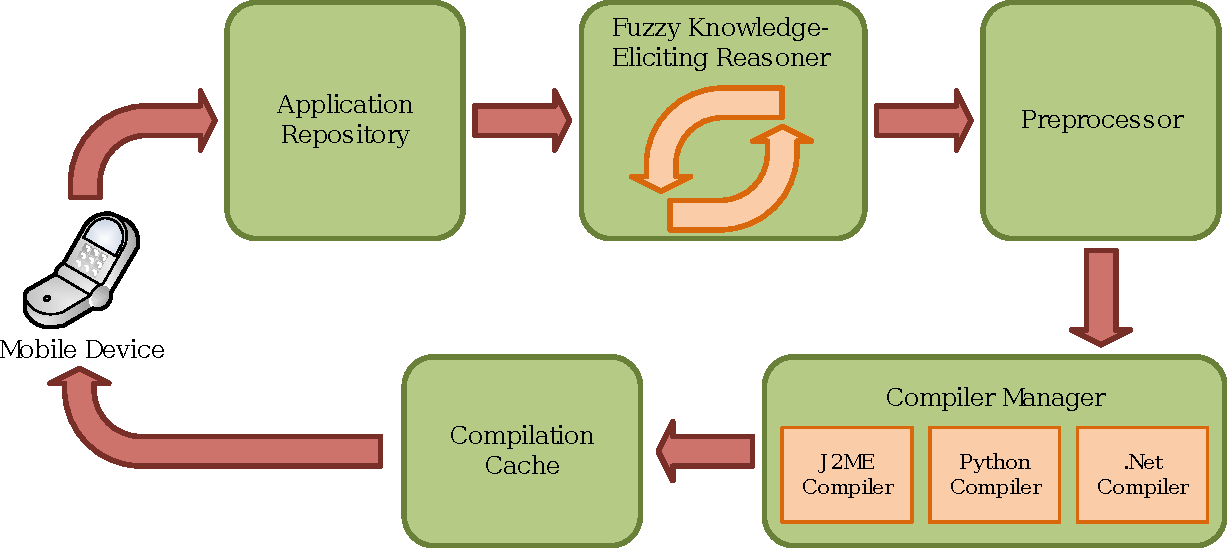
\includegraphics[width=0.90\textwidth]{imhotep_architecture.pdf}
\caption{The Imhotep architecture~\citep{imhotep_website}.}
\label{fig:imhotep_architecture}
\end{figure}

The preprocessor directives define how the final source code must be generated, 
providing conditions for certain regions of code to be added or skipped and 
adding the corresponding \ac{ui} variables that the preprocessor will adapt for each
compilation. The preprocessor identifies the directives when they start by //\#
in languages that support inline comments starting by //, such as Java, C\# or
C++, \#// in languages that support inline comments starting by \#, such as 
Python or Perl, and '// in VB.NET.

The preprocessor can avoid the compilation of fragments of code if certain 
conditions are met. These conditions can include calls to functions provided 
by the system. Basic string and \textit{math} functions are available, including
\textit{lowercase}, \textit{trim}, \textit{contains}, \textit{round} or 
\textit{sqrt}, as well as functions to check if a certain variable is 
available. The conditions can be embedded, as shown in the code below. The 
syntax of the conditions is  based on the syntax used by the Python programming 
language. The following code shows an example of using preprocessor directives 
in Java. During compiling time this code will be analysed by the framework 
taking into account the defined variables and their values. Therefore, the final 
binaries will contain just one reference to one of the methods shown in 
Listing~\ref{lst:preprocessor_directives}.


\inputminted[linenos=true, fontsize=\footnotesize, frame=lines]{python}{5_experiments_and_results/preprocessor_directives.py}
\captionof{listing}{Using the Imhotep framework through preprocessor 
directives~\citep{imhotep_website}.\label{lst:preprocessor_directives}}


Developers ask for user and device capabilities in these conditions. For 
example, one directive could state that if the user is blind the application 
should use a voice based interface. Five categories of user capabilities were 
defined (see Figure~\ref{fig:imhotep_user_capabilities}).


\begin{figure}
\centering
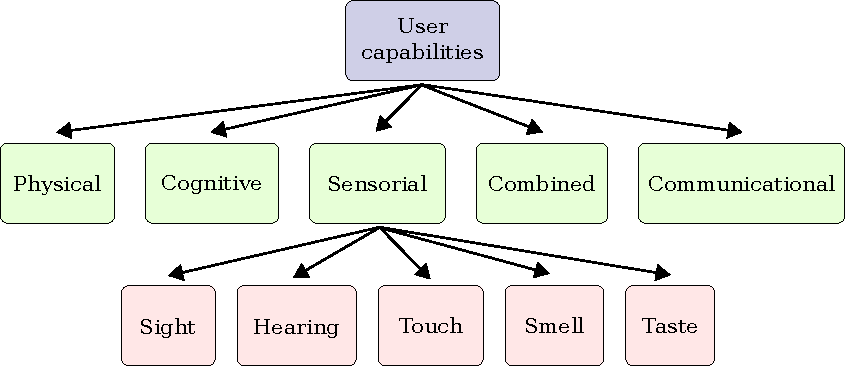
\includegraphics[width=0.90\textwidth]{imhotep_user_capabilities.pdf}
\caption{The set of Imhotep's user capabilities~\citep{imhotep_website}. As is
shown, user capabilities are classified into 5 different groups: physical, 
relative to user's motor skills; cognitive, which deals with memory and 
comprehension capabilities; sensorial, including capabilities related to 
sight, hearing, touch, smell and tast; combined, including combination of 
different disabilities; and communicational, which deals with speech.}
\label{fig:imhotep_user_capabilities}
\end{figure}

Now that the Imhotep framework has been introduced, a comparison between AdaptUI and
Imhotep running the same experiments is presented. Despite the fact that both solutions
have the same purpose (to help reducing the boundaries for those who cannot
properly interact with a user interface), their differences are substantial.
Imhotep directly depends on a server (allocated in the University of Deusto)
while AdaptUI runs fully in the mobile phone, performing the adaptation on the
fly. 

\subsubsection{Use Case: AssistedCity}
\label{sec:assisted_city_use_case}

As said before, Imhotep is a framework for developers which provides a 
preprocessor directive based procedure to build adaptive user interfaces. The 
Imhotep framework was originally tested with AssistedCity\footnote{\url{
https://github.com/aitoralmeida/imhotep/tree/master/PiramideRestServer/deploy/piramide/applications/AssistedCity/1.0.0.0/project}}. 
AssistedCity is a tour 
guide application which guides the user taking into account several points of interest 
categories (i.e., monuments, museums, restaurants, and so forth) that the user 
needs to choose from a menu. Then, using the camera and through an Augmented 
Reality interface the application guides the user to the desired point of 
interest. As a demonstrator of the Imhotep framework, this application was 
developed using several preprocessor directives which take into account sight 
sensory capabilities, hearing capabilities and device's screen size, to adapt 
the user interface of the application. Hence, we have chosen the same use case to 
evaluate the results of the adaptation using the corresponding platform.

This evaluation is split in two different parts. First, a visual comparison of
the resulting adaptations is shown. Then, we focus on the performance of both
solutions, specially on the required time to get the whole processes finished.

For the adaptation using Imhotep, an extra application is needed to send the 
user's and device's characteristics to the Imhotep server. 
Listing~\ref{lst:variables} shows the variables file used by Imhotep to perform
the corresponding adaptation. This file is completed by the user when he/she 
uses the cited application. Once the variables file is completed, the user is 
able to download the desired provided application from the Imhotep server.


\inputminted[linenos=true, fontsize=\footnotesize, frame=lines]{json}{5_experiments_and_results/variables.json}
\captionof{listing}{The variables file, in which device characteristics and user 
capabilities are described.\label{lst:variables}}


On the contrary, the corresponding AdaptUI models for the user and the device 
are represented  through the AdaptUIOnt ontology, and there is no need for 
external servers. The similar user and device situation is represented as 
follows, in Table~\ref{tbl:adaptui_repr}:

\begin{table}
 \caption{User and device characteristics representation in AdaptUIOnt.}
 \label{tbl:adaptui_repr}
 \footnotesize
 \centering
\begin{tabular}{l l l l }
\hline 
\textbf{Entity} & \textbf{Class}   & \textbf{Data property}  & \textbf{value}\\
\hline
\textit{User}&
\textit{Display} & \textit{userDisplayBrightnessIsStatic}  &\textit{false}\\
\textit{(UserCharacteristics)}& & \textit{userDisplayIsApplicable} 	   
&\textit{false}\\
&\textit{Audio} & \textit{userDisplayApplicableIsStatic}   &\textit{false}\\
&		 & \textit{userAudioHasApplicable} 	   &\textit{true} \\
&		 & \textit{userAudioApplicableIsStatic}    &\textit{false}\\
&		 & \textit{userAudioHasVolume}  	   & 5		  \\
&\textit{Interface}& \textit{userInterfaceInput} 	   &\textit{haptic}\\
&		 & \textit{userInterfaceOutput} 	   &\textit{default}\\
&\textit{Experience}& \textit{userHasExperience} 	   &\textit{high} \\
&\textit{View}	 & \textit{userViewIsStatic}		   &\textit{false}\\
&\textit{Other} 	 & \textit{userHasLanguage}		   
&\textit{English}\\
		 & \textit{vibration} 			   &\textit{true}\\
\hline
\textit{Device} & \textit{DeviceScreenResolution} & 
\textit{deviceHasScreenResolution} & 1280 x 720\\
\textit{(DeviceCharacteristics)} & \textit{OS} & \textit{deviceHasOSVersion} & 
4.3\\
\hline
\end{tabular}
\end{table}


The results of the adaptations are illustrated in the following figures. First,
Figure~\ref{fig:ac_default} shows the default user interface for the main menus 
of the application. It originally consists of several visual icons representing 
different venues categories (i.e., bars, restaurants, cafés, and so on). Once the 
user chooses one option, a list with the nearer corresponding type of venues
is presented.

\begin{figure}
\centering
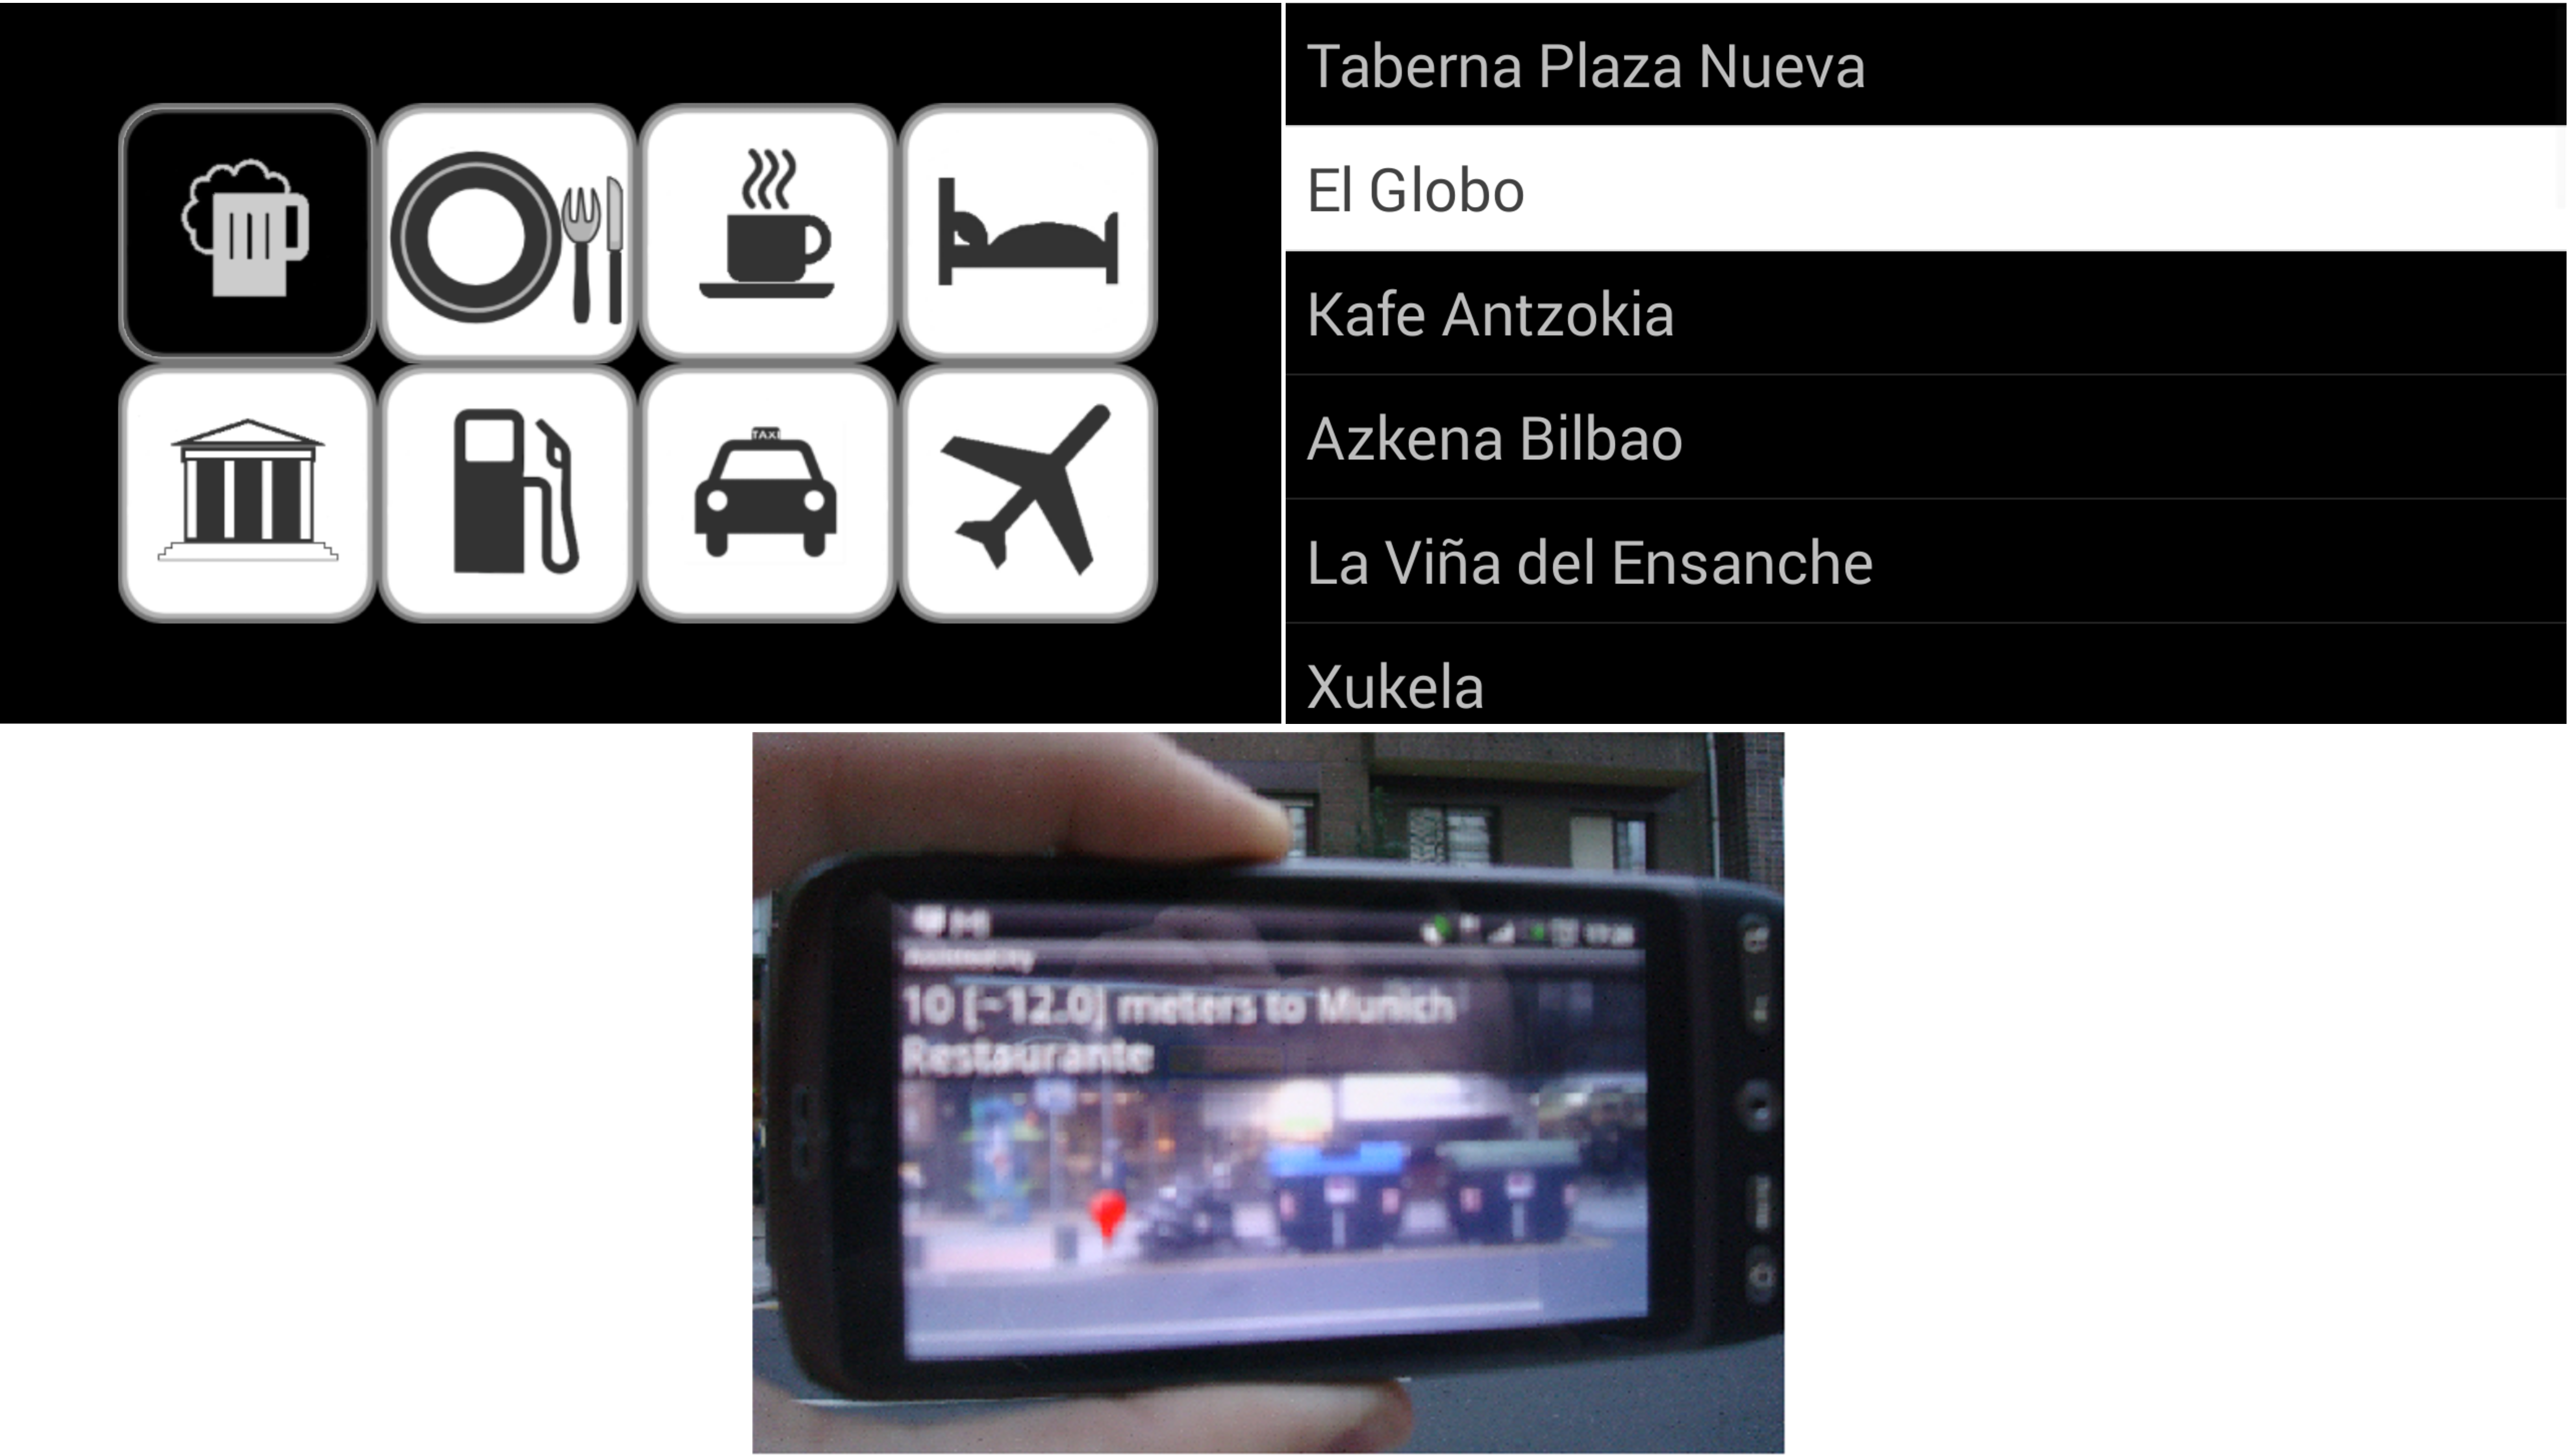
\includegraphics[width=0.75\textwidth]{ac_default.pdf}
\caption{AssistedCity default menus and user interface.}
\label{fig:ac_default}
\end{figure}

Next, a comparison between the two adaptations is illustrated through 
Figure~\ref{fig:ac_adapted}. On the left the adaptation performed by Imhotep is 
shown. The parameters detailed in Listing~\ref{lst:variables} for the user and 
device characteristics are sent to the Imhotep server. Then, the corresponding
application is generated and send back to the user. On the contrary, on the 
right side of Figure~\ref{fig:ac_adapted} there is the adaptation performed by 
AdaptUI. Considering the input detailed in Table~\ref{tbl:adaptui_repr} AdaptUI 
performs the corresponding adaptation (depending on the set of specified rules).
The adaptation performed by AdaptUI matches the input capabilities shown in
Table~\ref{tbl:adaptui_repr}, which represents better the user capabilities
than the specification given by Listing~\ref{lst:variables}.

\begin{figure}
\centering
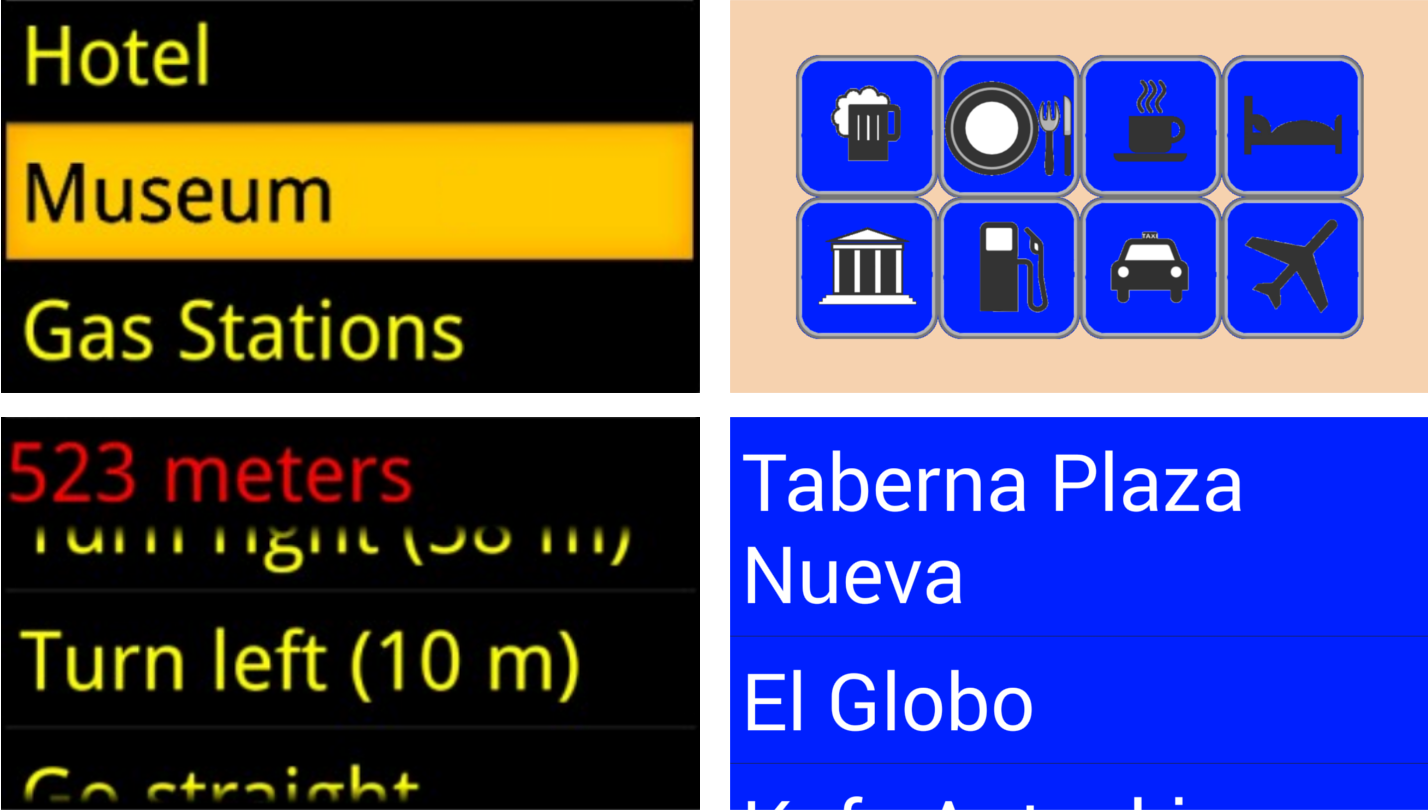
\includegraphics[width=0.60\textwidth]{ac_adapted.png}
\caption{AssistedCity adapted by Imhotep (left) and AdaptUI (right) taking 
into account the corresponding inputs shown in Listing~\ref{lst:variables} and 
Table~\ref{tbl:adaptui_repr}.}
\label{fig:ac_adapted}
\end{figure}


% the difference adaptation for the main menu of 
% the AssistedCity application. On the left, there is the adaptation performed by
% Imhotep using the parameters detailed in Listing~\ref{lst:variables} for the 
% user and device characteristics.

Regarding the time performance evaluation in Table~\ref{tbl:imhotep_timing}, it 
shows the time required by Imhotep to adapt AssistedCity. As seen through this 
table, if the server maintains a cache of the already adapted applications for 
the specific user and device the response of the system does not exceed 1.3
seconds. 

\begin{table}
 \caption{Imhotep framework time analysis. The figures under Mean, Median and
 standard deviation (Std. deviation) are represented in seconds.}
 \label{tbl:imhotep_timing}
 \footnotesize
 \centering
\begin{tabular}{l l l l l l l}
%  S[round-precision=2]
  \hline 
  \textbf{Device} & \multicolumn{3}{c}{\textbf{Cached 
  data}} & \multicolumn{3}{c}{\textbf{Non cached data}}\\
  & \textbf{Mean} & \textbf{Median} & \textbf{Deviation} &  \textbf{Mean} 
  & \textbf{Median} & \textbf{Deviation}\\
  \hline    
  Galaxy SIII~Mini & 1,257 & 1,237 & 0,247 & 15,125 & 15,034 & 0,445\\
%   
  Galaxy SIII & 1,175 & 1,107 & 0,239 & 15,094 & 14,950 & 0,501 	\\
%   
  Nexus 10 & 1,211 & 1,184 & 0,180 & 15,115 & 15,033 & 0,492 	\\
 \hline
\end{tabular}
\end{table}

On the contrary, AdaptUI does not require an external server, and it does not 
use any cache. Thus, the required time for the adaptation depends mostly on the 
hardware of the device running the reasoning process. Table~\ref{tbl:imhotep_vs_adaptui}
compares the means of using Imhotep or AdaptUI for an adaptation. In the case of 
AdaptUI, a light change in context triggers the process. Obviously, this represents
one of the most significant benefits of AdaptUI, as the platform is able to 
dynamically react to these changes. On the contrary, a user of AssistedCity will
need to indicate the new situation in the variables file, and the reasoning process
will start again in the Imhotep server.

\begin{table}
 \caption{Comparing Imhotep and AdaptUI time performance. The mean is 
represented in seconds.}
 \label{tbl:imhotep_vs_adaptui}
 \footnotesize
 \centering
\begin{tabular}{l l l l}
  \hline 
  \textbf{System} & \textbf{Platform} & \textbf{Cache/Trigger} & \textbf{Mean}\\
  \hline
  Imhotep 	& Galaxy SIII~Mini	& Cached		& 1.257\\
		&  			& Not cached		& 15.125\\
		& Galaxy SIII 		& Cached		& 1.211\\
		&  			& Not cached		& 15.115\\
		& Nexus 10 		& Cached		& 1.175\\
		&  			& Not cached		& 15.094\\
  \hline
  AdaptUI 	& Galaxy SIII~Mini	& Context change	& 1.899\\
		& Galaxy SIII		& Context change	& 1.544\\
 		& Nexus 10 		& Context change	& 1.213\\
  \hline
\end{tabular}
\end{table}

\subsubsection{Discussion}
\label{sec:imhotep_discussion}

Imhotep was conceived in 2010, when the hardware characteristics of the available 
Android devices was still limited. First 1 \ac{ghz} processors started to power 
these devices, and their \ac{ram} memory vaguely exceeded 500 \ac{mb}. Considering 
these limitations, Imhotep was designed following the same approach that several 
solutions cited in Chapter~\ref{cha:state_of_the_art} used: externalizing the 
computational complex processes to an external server. Hence, in Imhotep the 
developers have to use several available preprocessor directives where the user 
interface alternative code has to be included. Then, their source code is 
uploaded to an external server, which would generate the corresponding binaries 
(according to user's requests) with the corresponding adaptation. These requests 
include the characteristics of the mobile device and the user's profile. 

Although Imhotep was a good approximation as a tool for developers to write 
applications with adaptive user interfaces, we have found several problems
in it:

\begin{itemize}
  \item Regarding final users, \textit{Imhotep requires an extra tool for 
  downloading the required application} with the corresponding and adapted user 
  interface. This means that every time the user requires a different adaptation 
  the profile configuration process is launched. Thus, if there is no cached data 
  in the server, it will cause a significant delay in the adaptation process.
  
  \item Besides, \textit{Imhotep depends on Internet connection} for for the 
  adaptation, which might be problematic. As an external server is needed to 
  perform the adaptive operations and source code compiling, there is the 
  possibility of a server or network failure, which would obviously affect or 
  even cancel the whole process.
  
  \item \textit{Context is not taken into account for the adaptation}. Only the 
  user and the characteristics of the current device were considered. Several 
  examples of the benefits of including context for the adaptation process have
  been presented during this section.
\end{itemize}

On the contrary, AdaptUI was conceived during 2013, when multi-core kernels and
CPUs were already deployed into mobile devices. These new characteristics 
increased their capabilities, making possible more complex processing. 
Therefore, AdaptUI first designs were definitely based on Android. This brings 
the whole adaptation process to the mobile. This means that, on the one hand, 
there is the advantage of not depending on the network or an external server to 
process anything. But it also means that the workload has to be managed by a 
hardware not as powerful or capable as a computer's one. As also detailed in 
Table~\ref{tbl:imhotep_vs_adaptui}, the adaptation performance relies on the
each device's hardware capabilities. 

Besides, AdaptUI includes the current context situation in the equation for the 
user interface adaptation. This fact presents several challenges and possibilities, 
as is considered in AdaptUI as a trigger for different situations involving the 
user and the device.


\subsubsection{Conclusions}
\label{sec:imhotep_conclusions}

During this section a comparison between AdaptUI and Imhotep has been performed.
Imhotep is a framework for easing the adaptation of user interfaces. In the 
presented figures and tables both solutions evaluation has been illustrated. 
The resulting adapted interfaces and the corresponding performance of both 
platforms have been shown. Next, we summarize our experiences through this 
evaluation with several considerations in the following lines.

As Imhotep needs an external server for the complex processing of the user 
interface adaptations, maintaining a cache is vital for this system. On the 
contrary, and as shown in Table~\ref{tbl:imhotep_timing}, the response time 
from rebuilding the whole source code results in a 15 seconds delay. Comparing with
the cached results, which imply less than 1.5 seconds to perform the same 
operation is clear that the difference is significant. Nevertheless, one of the 
benefits of this solution is that, as the adaptation process is delegated to an 
external server, is not important which device is being used by the user. The
current device has just to be compatible with the applications available in the
server.

One of the main problems of Imhotep is that context is not taken into account 
for the adaptations. The explanation for this decision was based on the time 
limitation of Imhotep for performing a complete adaptation. 
Figure~\ref{fig:imhotep_comparison} illustrates how operating without cached 
data takes around 15 seconds for receiving the corresponding user interface in 
the device. This means that the context might change during this period of time. 
On the other side, the cache was conceived to store information about the 
profile of the user and the device that might not change during time. By using 
this cache the adaptations were sent back to the device in less than 2 seconds.

\begin{figure}
\centering
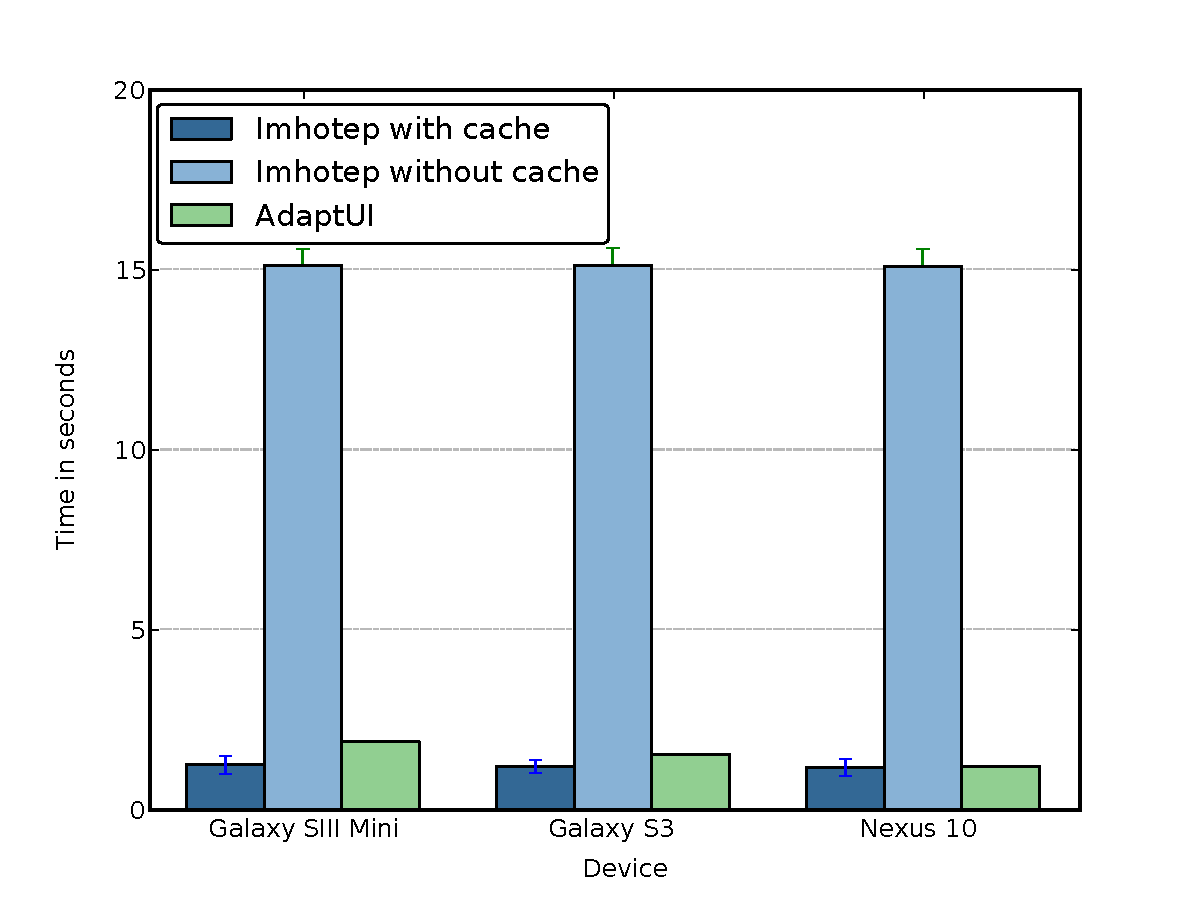
\includegraphics[width=0.75\textwidth]{imhotep_comparison.pdf}
\caption{Receiving the corresponding adapted user interface for different
devices using Imhotep without cache.}
\label{fig:imhotep_comparison}
\end{figure}


Imhotep time responses are obtained as the result of the addition of three
different processes. The first one is the required time in terms of networking,
that takes to send the adaptation request from the device to the adaptation 
server. Secondly, the required time to process the request, compile and generate 
the adapted version (around 14 seconds). And finally, the time needed to send 
the adaptation back to the user's device with the corresponding user interface. 

On the other hand, AdaptUI performance does not depend on the network traffic, 
as it runs fully in the mobile device. Thus, the obtained performance results 
depend only on the hardware and software capabilities of the device. The 
triggers are launched by the user for Imhotep and by a context change for 
AdaptUI respectively. This is shown in Table~\ref{tbl:imhotep_vs_adaptui}.

Regarding the presented arguments, we conclude that:

\begin{enumerate}[label=\alph*)]
  \item Imhotep's performance when using a cache is similar (even better) when
  network conditions are optimal. 
  
  \item As Imhotep does not carry out complex operations in the mobile devices,
  leaving this workload to an external server, the hardware specifications of 
  the current device are not as important as in AdaptUI.
  
  \item On the contrary, this dependency carries several drawbacks. For 
  example, a network failure would leave the adaptation process incomplete.
  
  \item Besides, although working with a cache results in similar time responses
  than AdaptUI, first adaptations of each application will cost a high time to
  be performed. During this time (around 15 seconds under normal circumstances)
  the context of the user might change, and it is possible for the user to 
  reject the adaptation.
  
  \item As AdaptUI takes the context into account, the adapted solutions are
  more characterized for the current user situation.
  
  \item Although depending on the device's hardware, it might result into slower
  adaptations, managing small semantic models (as AdaptUIOnt) is still 
  manipulable by the platform. Besides, as the smartphones market grows in terms
  of hardware capabilities, the performance of such systems will be increased.
  
  \item AdaptUI does not consider explicit physiological user capabilities. On 
  the contrary, Imhotep works with a user model in which it is necessary to
  provide several physiological based capabilities. This results into a non
  practical solution, as we lack medical knowledge.
  
  \item Another benefit from AdaptUI is the automation of the adaptation 
  through several sets of adaptation rules. These rules, not considering 
  explicit physiological user capabilities, infer knowledge about the user that
  is vital for the adaptation. The whole set of rules that manages the adaptation
  process in AdaptUI are detailed in Section~\ref{sec:adaptui_rules}.
\end{enumerate}